\documentclass[a5paper,11pt]{extarticle}

\def\labauthors{Сарафанов Ф.Г., Платонова М.В.}
\def\labgroup{440}
\def\labnumber{1}
\def\labstartdate{5 марта}
\def\labtheme{Исследование влияния\\[-0.2em] пространственного заряда\\[0.2em] на
прохождение тока в диоде}
\def\shortlabtheme{Вакуумный диод}

%!TEX root = ../vdiode.tex
\usepackage{cmap}
\usepackage[T2A]{fontenc}
\usepackage[utf8x]{inputenc}
\usepackage[english, russian]{babel}

\usepackage{misccorr} % в заголовках появляется точка, но при ссылке на них ее нет
\usepackage{amssymb,amsfonts,amsmath,amsthm}  
\usepackage{indentfirst}
\usepackage[usenames,dvipsnames]{color} 
\usepackage[unicode,hidelinks]{hyperref}
% \hypersetup{%
%     pdfborder = {0 0 0}
% }

\usepackage{makecell,multirow} 
\usepackage{ulem}
\usepackage{graphicx,wrapfig}
\graphicspath{{img/}}
\usepackage{geometry}
\geometry{left=1.5cm,right=1.5cm,top=2cm,bottom=2cm,bindingoffset=0cm,headheight=15pt}
\usepackage{fancyhdr} 
\linespread{1.05} 
\frenchspacing 
\renewcommand{\labelenumii}{\theenumii)} 
\newcommand{\mean}[1]{\langle#1\rangle}
% \usepackage{caption}
%%%%%%%%%%%%%%%%%%%%%%%%%%%%%%%%%%%%%%%%%%%%%%%%%%%%%%%%%%%%%%%%%%%%%%%%%%%%%%%
%%%%%%%%%%%%%%%%%%%%%%%%%%%%%%%%%%%%%%%%%%%%%%%%%%%%%%%%%%%%%%%%%%%%%%%%%%%%%%%



%%%%%%%%%%%%%%%%%%%%%%%%%%%%%%%%%%%%%%%%%%%%%%%%%%%%%%%%%%%%%%%%%%%%%%%%%%%%%%%
	%применим колонтитул к стилю страницы
\pagestyle{fancy} 
	%очистим "шапку" страницы
\fancyhead{} 
	%слева сверху на четных и справа на нечетных
\fancyhead[L]{\labauthors} 
	%справа сверху на четных и слева на нечетных
\fancyhead[R]{\shortlabtheme} 
	%очистим "подвал" страницы
\fancyfoot{} 
	% номер страницы в нижнем колинтуле в центре
\fancyfoot[C]{\thepage} 
\renewcommand{\phi}{\varphi}
%%%%%%%%%%%%%%%%%%%%%%%%%%%%%%%%%%%%%%%%%%%%%%%%%%%%%%%%%%%%%%%%%%%%%%%%%%%%%%%

\usepackage{float}
\usepackage[mode=buildnew]{standalone}
\usepackage{tikz} 
% \usepackage{subcaption}
\usepackage{csvsimple}
\usetikzlibrary{scopes}
\usetikzlibrary{%
     decorations.pathreplacing,%
     decorations.pathmorphing,%
    patterns,%
    calc,%
    scopes,%
    arrows,%
    % arrows.spaced,%
}
\makeatletter
\newif\if@gather@prefix 
\preto\place@tag@gather{% 
  \if@gather@prefix\iftagsleft@ 
    \kern-\gdisplaywidth@ 
    \rlap{\gather@prefix}% 
    \kern\gdisplaywidth@ 
  \fi\fi 
} 
\appto\place@tag@gather{% 
  \if@gather@prefix\iftagsleft@\else 
    \kern-\displaywidth 
    \rlap{\gather@prefix}% 
    \kern\displaywidth 
  \fi\fi 
  \global\@gather@prefixfalse 
} 
\preto\place@tag{% 
  \if@gather@prefix\iftagsleft@ 
    \kern-\gdisplaywidth@ 
    \rlap{\gather@prefix}% 
    \kern\displaywidth@ 
  \fi\fi 
} 
\appto\place@tag{% 
  \if@gather@prefix\iftagsleft@\else 
    \kern-\displaywidth 
    \rlap{\gather@prefix}% 
    \kern\displaywidth 
  \fi\fi 
  \global\@gather@prefixfalse 
} 
\newcommand*{\beforetext}[1]{% 
  \ifmeasuring@\else
  \gdef\gather@prefix{#1}% 
  \global\@gather@prefixtrue 
  \fi
} 
\makeatother

\usepackage{booktabs}
\usepackage{pgfplots, pgfplotstable}

\usepackage[outline]{contour}
\usepackage{tocloft}
\renewcommand{\cftsecleader}{\cftdotfill{\cftdotsep}} % for parts
% \renewcommand{\cftchapleader}{\cftdotfill{\cftdotsep}} % for chapters
\usepackage{pgfplots,pgfplotstable,booktabs,colortbl}
\pgfplotsset{compat=newest}
\usepackage{physics}
\usepackage{mathtools}
\mathtoolsset{showonlyrefs=true}
\newcommand\Smat{\hat { \mathbf { S } }}

\newcommand*\dotvec[1][1,1]{\crossproducttemp#1\relax}
\def\crossproducttemp#1,#2\relax{{\qty[\vec{#1}\times\vec{#2}\,]}}

\newcommand*\prodvec[1][1,1]{\crossproducttempa#1\relax}
\def\crossproducttempa#1,#2\relax{{\qty[{#1}\times{#2}\,]}}

% \def\E{\mathscr{E}_H}
\def\Rdim{\,\frac{\text{м}^3}{\text{А} \cdot \text{с}}}

\renewcommand{\vec}{\mathbf} % for parts
\begin{document}
%!TEX root = ../diode.tex
\begin{titlepage}
\begin{center}
% \vspace{-3em}
{\small\textsc{Нижегородский государственный университет имени Н.\,И. Лобачевского}}
\vskip 2pt \hrule \vskip 3pt
{\small\textsc{Радиофизический факультет}}

\vfill


{{\large Отчет по лабораторной работе №\labnumber}\vskip 12pt {\LARGE \bfseries \labtheme}}

	
\vspace{2cm}
{\large Работу выполнили студенты \\[-0.25em] \labgroup\  группы радиофизического факультата \\[0.5em] {\Large \bfseries \labauthors}}

% \vspace{0.5cm}
% {e-mail: sfg180@yandex.ru}

% \vspace{2cm}

\end{center}

\vfill
	
% \begin{flushright}
% 	{Выполнили студенты 430 группы\\ \labauthor}%\vskip 12pt Принял:\\ Менсов С.\,Н.}
% \end{flushright}
	
% \vfill
	
\begin{center}
	{Нижний Новгород, \labstartdate\ -- \today}
\end{center}

\end{titlepage}

\tableofcontents
\newpage



\addcontentsline{toc}{section}{Введение}
\section*{Введение}
\vspace{-0.5em}
В настоящей работе изучается \textit{вакуумный диод}. В качестве активной излучающей среды выступают интенсивные электронные потоки, процессы в которых существенно зависят от собственного кулоновского поля пучка. Изучение вакуумного диода позволяет теоретически найти распределение потенциала, влияние пространственного заряда на процессы протекания тока в диоде, вольт-амперную характеристику диода. 

В работе используется упрощенная теория диода, описывающая процессы в диоде с плоской симметрией.



\vspace{-0.5em}
 % Как показано в \cite[стр. ы]{met}

\paragraph{Установка.} Установка представляет собой трёханодный диод, запитанный от источников постоянного тока и напряжения. Измеряемые и/или устанавливаемые величины: анодный ток диода, анодное напряжение, ток и напряжение накала катодной цепи.

В работе снимается вольт-амперная зависимость при различных схемах подключения цепи накала к анодной цепи: минус анодного источника питания на минусе цепи накала, минус анодного источника на плюсе цепи накала, и симметричная схема включения -- с помощью симметричного делителя напряжения, включенного параллельно цепи накала.

Так же снимается зависимость анодного тока от тока накала, что позволяет рассчитать (используя известную зависимость температуры нити от тока накала) работу выхода вольфрамового катода.

\newpage

% \newpage

\section{Эксперимент}
\subsection{Вольт-амперные характеристики диода}
\subsubsection{Схема 1}
Измерение ВАХ проводится при подключении установки, отвечающем принципиальной схеме, приведенной на рис. \ref{fig:chem1}. При этом задается фиксированное значение тока накала $i_\text{нак}=1.480$ А, а ВАХ снимается в диапазоне напряжений от 0 до 120 В (рис. \ref{fig:vax1}).
\begin{figure}[H]
	\centering
	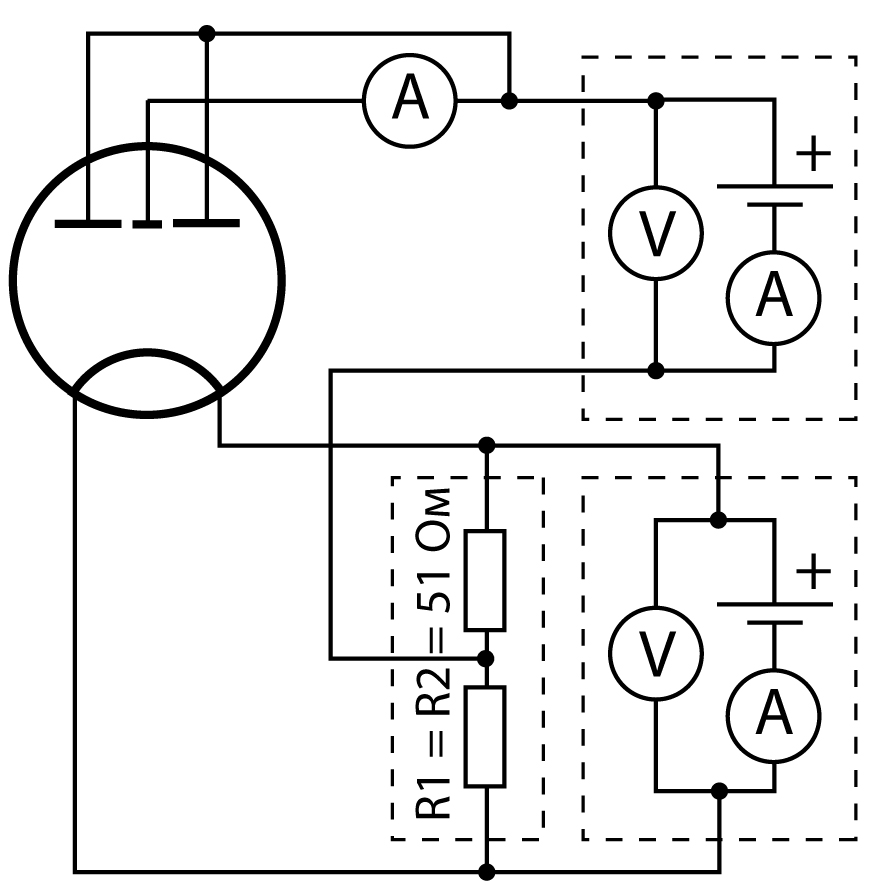
\includegraphics[width=0.3\textwidth]{img/z1.jpg}
	\vspace{-1em}
	\caption{Схема экспериментальной установки №1}
	\label{fig:chem1}
\end{figure}

\begin{figure}[H]
	\centering
	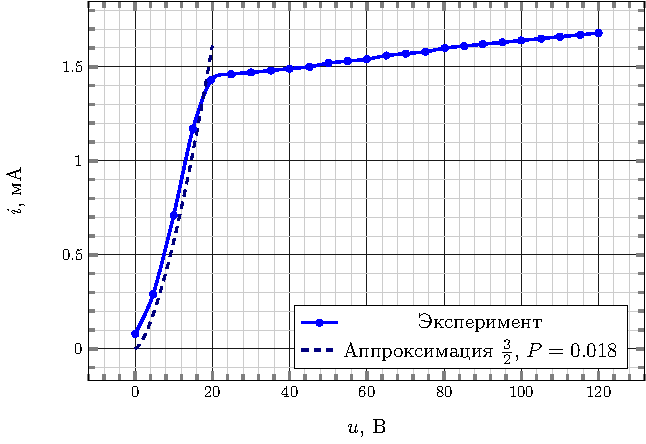
\includegraphics[scale=0.9]{fig/i_from_u_1.pdf}
	\vspace{-1em}
	\caption{ВАХ при подключении по схеме №1, ток накала 1.480 А}
	\label{fig:vax1}
\end{figure}

Начальный участок вольт-амперной характеристики (до 20 вольт) аппроксимировался законом трех вторых, при этом первеанс составил
\begin{equation}
	P=18\cdot 10^{-3} \,\,\frac{\text{мА}}{\text{В}^{\frac32}}.
\end{equation}
Отсюда по формуле для цилиндрического диода
\begin{equation}
J_a=\frac49 \varepsilon_0 \sqrt{2 \eta} \frac{S_a}{r_a^2 \beta^2} U^{3/2}, 
\end{equation}
где $\beta^2\approx(1-\frac{r_k}{r_a})^2$, $r_a$= 0.4 см, $r_k$= 0.005 см, $S_a\approx 8 \text{ см}^2$ -- площадь анода, находится  удельный заряд электрона: 
\begin{equation}
	\eta=2.6 \cdot 10^{11} \,\,\frac{\text{кл}}{\text{кг}}.
\end{equation}

\newpage
\subsubsection{Схема 2}
Установка,подключалась следующим образом (см. рис. \ref{fig:chem2}). При фиксированном значении тока накала $i_\text{нак}=1.500$ А снята ВАХ в диапазоне напряжений от 0 до 120 В (рис. \ref{fig:vax2}).
\begin{figure}[H]
	\centering
	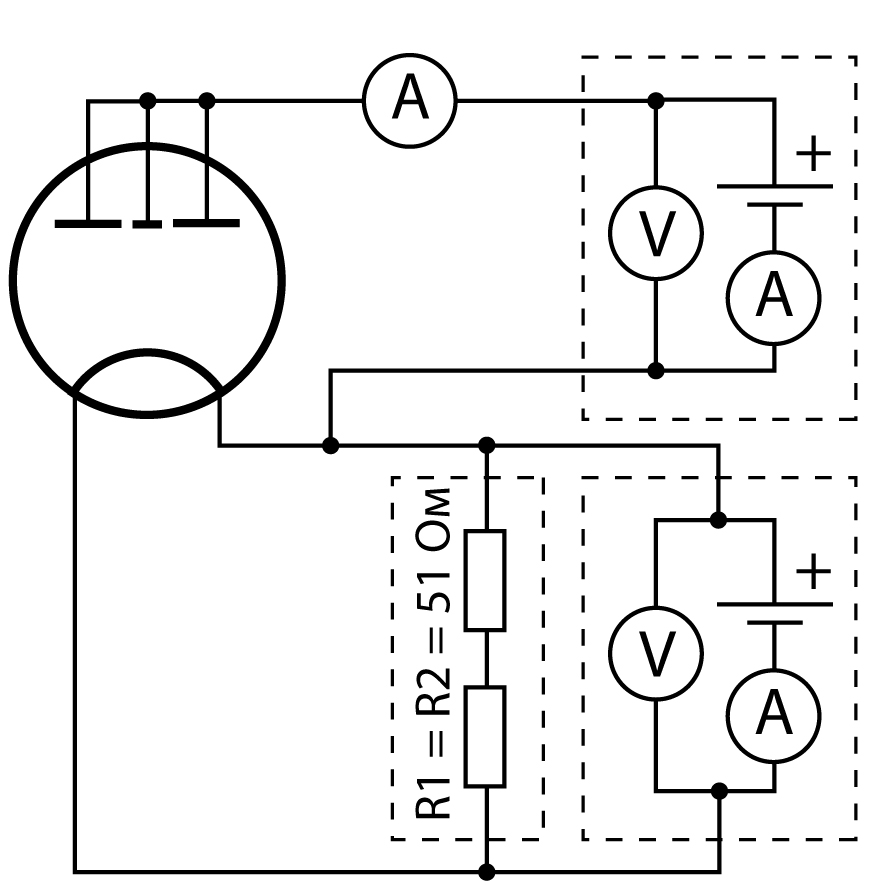
\includegraphics[width=0.3\textwidth]{img/z2.jpg}
	\vspace{-1em}
	\caption{Схема экспериментальной установки №2}
	\label{fig:chem2}
\end{figure}

\begin{figure}[H]
	\centering
	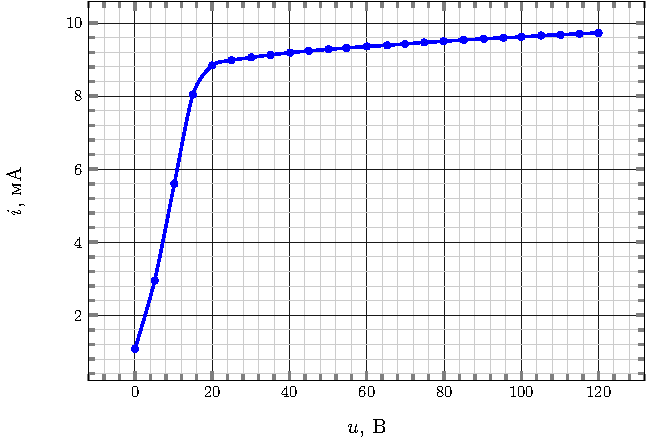
\includegraphics[]{fig/i_from_u_2.pdf}
	\vspace{-1em}
	\caption{ВАХ при подключении по схеме №2, ток накала 1.500 А}
	\label{fig:vax2}
\end{figure}

\subsubsection{Схема 3}
На установке, собранной  по схеме, изображенной на рис. \ref{fig:chem3}, снята ВАХ в диапазоне напряжений от 0 до 120 В (рис. \ref{fig:vax3}) при трех различных фиксированных значениях тока накала: 1.420, 1.460 и 1.500 ампер. Для каждого значения тока фиксировалось значение напряжения накала (см. рис. \ref{fig:vax3}).
\begin{figure}[H]
	\centering
	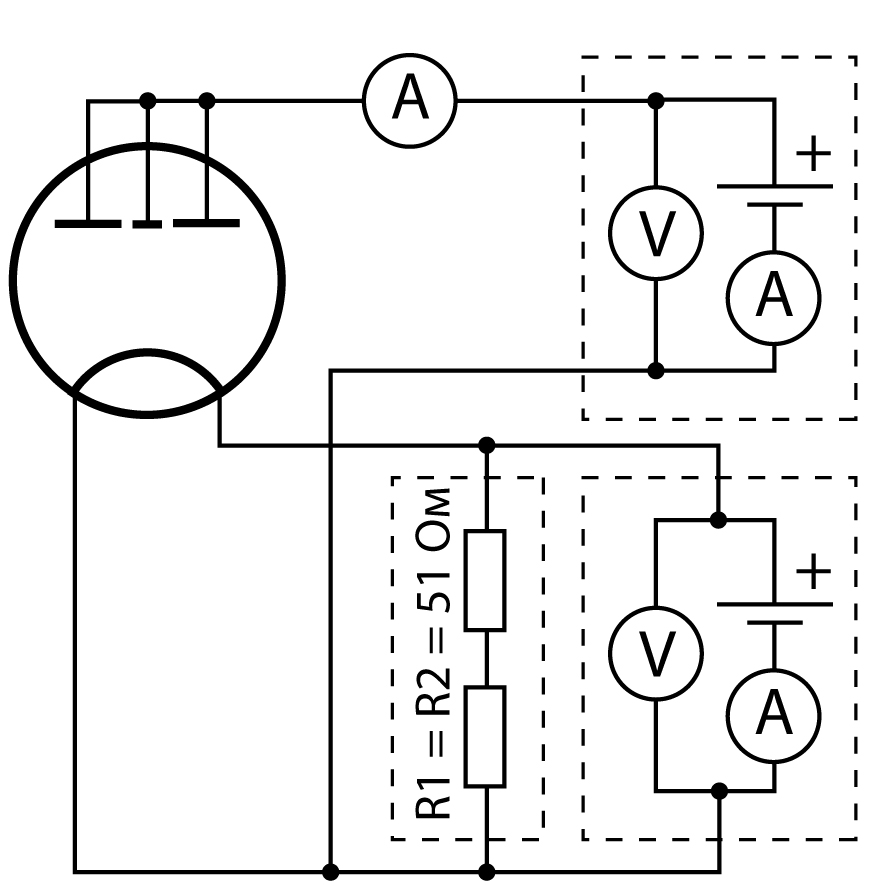
\includegraphics[width=0.3\textwidth]{img/z3.jpg}
	\vspace{-1em}
	\caption{Схема экспериментальной установки №3}
	\label{fig:chem3}
\end{figure}
\begin{figure}[H]
	\centering
	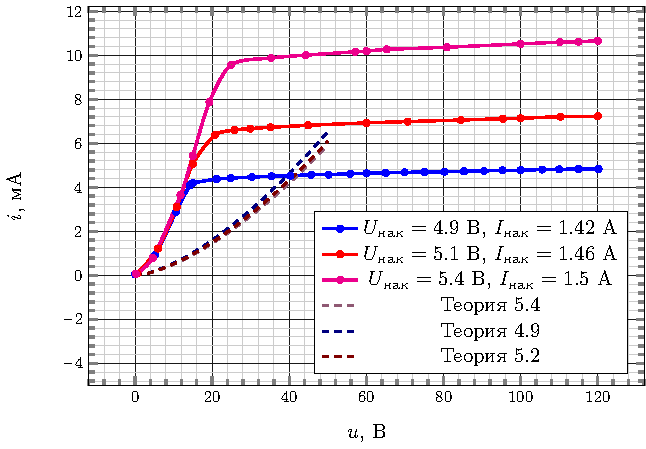
\includegraphics[]{fig/i_from_u_3.pdf}
	\vspace{-1em}
	\caption{ВАХ при подключении по схеме №3}
	\label{fig:vax3}
\end{figure}

Для всех трех зависимостей также рассчитана и построена теоретическая зависимость с помощью таблицы $F(u_a/u_f)$.

\subsection{Зависимость анодного тока от тока накала}
 При трех фиксированных анодных напряжениях (15, 60, 100 вольт) снята зависимость анодного тока от тока накала\footnote{Максимальный ток накала 1.5 ампер} (рис. \ref{fig:iia}). Измерения проводились на установке, собранной по схеме 3 (рис. \ref{fig:chem3}).
\begin{figure}[H]
	\centering
	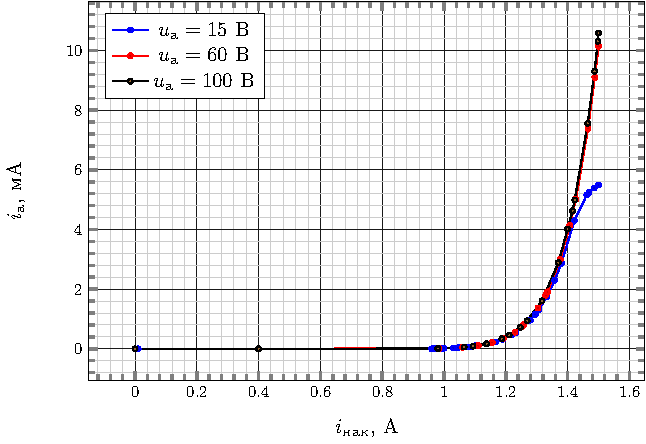
\includegraphics[]{fig/i_from_ia.pdf}
	\caption{Зависимость $i_a(i_\text{нак})$}
	\label{fig:iia}
\end{figure}

C хорошей точностью зависимость температуры от тока накала (из таблицы Люнгмера) аппроксимируется линейной зависимостью
\begin{equation}
	T(i_\text{нак})=970.52+996.208\cdot i_\text{нак}.
\end{equation}
С помощью такого приближения рассчитывается температура для каждого значения накала и строится прямая Ричардсона (рис. \ref{fig:rich}):
\begin{equation}
	\ln i_a -2\ln T = \ln(S_a\cdot A) - \frac{e\varphi}{kT},
\end{equation}
по наклону которой определяется работа выхода.
\begin{figure}[H]
	\centering
	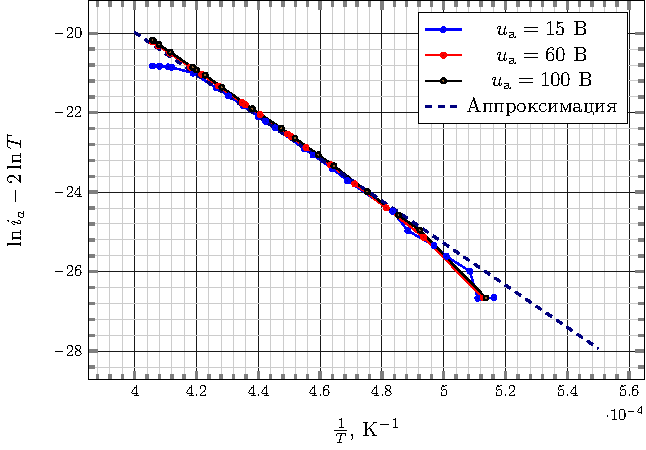
\includegraphics[]{fig/richardson.pdf}
	\caption{Прямая Ричардсона}
	\label{fig:rich}
\end{figure}
\vspace{-0.5em}
Из графика определена работа выхода по наклону графика на линейном участке для вольфрамового катода
\begin{equation}
	A_\text{вых}=5.3 \text{ эВ}.
\end{equation}


\addcontentsline{toc}{section}{Заключение}
\section*{Заключение}
В настоящей работе мы изучили принципы работы вакуумного диода, измерили основные характеристики диода при различных схемах подключения цепи накала, получили прямую Ричардсона, откуда нашли работу выхода катода.

% \begin{thebibliography}{}
%   \bibitem{orlov} Орлов И.\,Я., Односевцев В.\,А. и др. Основы радиоэлектроники: учебное пособие. -- Нижний Новгород: Нижегородский государственный университет им. Н.И. Лобачевского, 2011. -- 169 с.
  
%   \bibitem{met} Битюрин\,\,Ю.\,А. и др. Измерение статических характеристик полупроводникового диода. Н.Новгород: ННГУ, 2004. -- 38 с.
  
%   % \bibitem{lit3} Ландау Л.Д., Лифшиц Е.М. Любой том. М.: Физматлит, 2003.
% \end{thebibliography}
\end{document}